\documentclass[a4paper]{article}
\usepackage[english]{babel}
\usepackage[utf8x]{inputenc}
% package for including graphics with figure-environment
\usepackage{graphicx}
\usepackage{parskip}
\usepackage{amssymb}
\usepackage{mathbbol}
\usepackage{eurosym}
\usepackage{amsmath}
\DeclareMathOperator*{\minimize}{minimize}
%\usepackage{verbatim}
\usepackage{hyperref}
\usepackage[natbibapa]{apacite}
\usepackage{geometry}
\geometry{
 a4paper,
 %total={170mm,257mm},
 left=30mm,
 top=30mm,
 right = 20mm,
 bottom = 30mm
 }
% colors for hyperlinks
% colored borders (false) colored text (true)
\hypersetup{colorlinks=true,citecolor=black,filecolor=black,linkcolor=black,urlcolor=black}

% package for bibliography
\PassOptionsToPackage{authoryear,round}{natbib}
% package for header
\usepackage[automark]{scrpage2}
\usepackage{braket}
\usepackage{enumerate}
\pagestyle{scrheadings}
\usepackage{ragged2e}
\ihead[]{Mark Fingerhuth}
\ohead[]{\today}
\cfoot[]{\pagemark} 
\setheadsepline[160mm]{0.3mm}

% Defining some new mathematics commands
\newcommand*{\colvec}[1]{\begin{pmatrix}#1\end{pmatrix}}
\newcommand*{\0}{$\ket{0}$}
\newcommand*{\1}{$\ket{1}$}


\begin{document}
\title{
\vspace{0.5cm}
\begin{figure}[!ht]
\centering

\includegraphics[width=0.5\textwidth]{MSC2.png}
\end{figure}
\vspace{0.3cm}
\begin{figure}[!ht]
\centering

\includegraphics[width=0.5\textwidth]{logo.jpeg}
\end{figure}
\vspace{1.6cm}
\Huge{ \underline{Research Proposal} \\ \vspace{1cm} \bf Proof-of-Concept Implementation of Quantum Machine Learning Algorithms \\ \vspace{1cm}}}
% Insert here your name and correct mail address
\author{\Large \href{mailto:m.fingerhuth@student.maastrichtuniversity.nl}{Mark Fingerhuth}
}
\date{
\today \\
\vspace{1.0cm}
\footnotesize{
In partial fulfillment of the requirements for the degree Bachelor of Science (BSc) at Maastricht University. \\}
\vspace{3.5cm}
\normalsize
In collaboration with the Quantum Research Group at the University of KwaZulu-Natal Durban. Under supervision of Prof. Francesco Petruccione, Quantum Research Group at UKZN, and internal supervision of Dr. Fabrice Birembaut, Maastricht Science Programme, Maastricht University.
}
% In partial fulfillment of the requirements for the degree Bachelor of Science, Maastricht University. 
\maketitle
\setlength{\parindent}{0pt}

%Braket package: $\braket{0|0}$

\vspace{10.0cm}
\begin{abstract}
\noindent Quantum machine learning, the intersection of quantum computation and classical machine learning, bears the potential to provide more efficient ways to deal with big data through the use of quantum superpositions, entanglement and the resulting quantum parallelism. The proposed research will attempt to implement and simulate two quantum machine learning routines and use them to solve small machine learning problems. That will establish one of the earliest proof-of-concept studies in the field and demonstrate that quantum machine learning is already implementable on small-scale quantum computers. This is vital to show that an extrapolation to larger quantum computing devices will indeed lead to vast speed-ups of current machine learning algorithms.

%bears the potential to resolve the problems in classical machine learning such as the growing computational complexity

\end{abstract}
	\newpage
	\tableofcontents
	\newpage

\section{Introduction}
\label{sec:introduction}

%>> Introduce the TOPIC (QML) not the (HYPO)THESIS!

The ability to understand spoken language, to recognize faces and to distinguish types of fruit comes naturally to humans, even though these processes of pattern recognition and classification are inherently complex. Machine learning (ML), a subtopic of artificial intelligence, is concerned with the development of algorithms that perform these types of tasks, thus enabling computers to find and recognise patterns in data and classify unknown inputs based on previous training with labelled inputs. Such algorithms make the core of e.g. human speech recognition and recommendation engines as used by Amazon.
% and algorithms that can predict heart disease from real-time electrocardiograms \citep{acharya2015integrated, pazzani2007content}.

According to \cite*{bigdata}, approximately 2.5 quintillion (${10}^{18}$) bytes of digital data are created every day. This growing number implies that every area dealing with data will eventually require advanced algorithms that can make sense of data content, retrieve patterns and reveal correlations. However, most ML algorithms involve the execution of computationally expensive operations and doing so on large data sets inevitably takes a lot of time \citep{bekkerman2011scaling}. Thus, it becomes increasingly important to find efficient ways of dealing with big data.
%and/or reduce the computational complexity of the algorithms.

A promising solution is the use of quantum computation which has been researched intensively in the last few decades. Quantum computers (QCs) use quantum mechanical systems and their special properties to manipulate and process information in ways that are impossible to implement on classical computers. The quantum equivalent to a classical bit is called a quantum bit (qubit) and additionally to being in either state \0 or \1 it can be in their linear superposition:
\begin{equation}
\label{equ: simplequbit}
\ket{q} = \alpha \ket{0} + \beta \ket{1}
\end{equation}
where $\alpha$ and $\beta$ are complex numbers and often referred to as amplitudes. When measuring qubit $\ket{q}$ it will take the value \0 with a probability of ${|\alpha|}^{2}$ and \1 with a probability of ${|\beta|}^{2}$. Since the total probability has to sum to unity, the normalization condition ${|\alpha|}^{2} + {|\beta|}^{2} =  1$ must be satisfied at all times.

This peculiar property gives rise to so-called quantum parallelism, which enables the execution of certain operations on many quantum states at the same time. Despite this advantage, the difficulty in quantum computation lies in the retrieval of the computed solution since a measurement of a qubit collapses it into a single classical bit and thereby destroys information about its previous superposition. Several quantum algorithms have been proposed that provide exponential speed-ups when compared to their classical counterparts with Shor's prime factorization algorithm being the most famous \citep{shor1994}.
%As another example, Grover's quantum database search algorithm enables finding a single element in a list of $N$ elements within roughly $\sqrt{N}$ quantum mechanical steps instead of $N$ classical steps \citep{grover}.
Hence, quantum computation has the potential to vastly improve computational power, speed up the processing of big data and solve certain problems that are practically unsolvable on classical computers. 

%for the QML toolbox to be complete a quantum algorithm to solve systems of linear equations is needed since most ML algorithms rely on solving those.

Considering these advantages, the combination of quantum computation and classical ML into the new field of quantum machine learning (QML) seems almost natural. There are currently two main ideas on how to merge quantum computation with ML, namely a) running the classical algorithm on a classical computer and outsourcing only the computationally intensive task to a QC or b) executing the quantum version of the entire algorithm on a QC. Current QML research mostly focusses on the latter approach by developing quantum algorithms that tap into the full potential of quantum parallelism.

%However, since most ML algorithms rely on solving some system of linear equations, a corresponding quantum algorithm is required for QML to become achievable. \cite{HHL2009} were first to describe a quantum algorithm solving linear equations of the form $A \cdot x = b$ exponentially faster than classical routines. This so called HHL algorithm has since become a subroutine in many QML algorithms. 


%QML
%- the unification or symbiosis of ML and QC comes naturally when considering the vast speed-ups that could be gained through implementing ML on QCs
%- this relatively new research field is called QML and is largely based on the discovery of the HLL algorithm
%- two possibilities: 1. run entire algorithm on QC or 2. run computationally exhaustive subroutines on QC and the rest on a CC


%ML

%- machine learning as a subarea of artificial intelligence is all about teaching/training a computer on how to recognise patterns, classify unknown information and ultimately learn from given input data
%- important for prediction algorithms, recommendation engines, expert machines (e.g. Watson) and computer vision or speech recognition
%- cite the amount of data humans create per year >> this huge amount of data requires advanced analysis in order to make sense of it
%- machine learning algorithms are usually very computationally exhaustive and when increasing the amount of data the computation time increases (exponentially???) >> maybe give the example of how long it took AlphaGo to be trained

%Quantum

%- quantum computation has become a very promising research area
%- it exploits/uses quantum mechanical systems to manipulate information and since quantum mechanics allows for superpositions it makes quantum parallelism possible / things like interference can be used to our benefit
%- offers the possibility of vastly boosting our computational power and enrich the space of solvable problems e.g. optimization problems (might be able to solve some P and NP problems) >> check this exactly
%- quantum mechanics essentially is 'applied linear algebra in complex vector spaces' and since classical computation is all about manipulating vectors and matrices the usefulness of QM for computation becomes obvious

\newpage

\subsection{Motivation}
\label{subsec:motivation}

Classical ML is a very practical topic since it can be directly tested, verified and implemented on any commercial classical computer. So far, QML has been of almost entirely theoretical nature since the required computational resources are not in place yet. To yield reliable solutions QML algorithms often require a relatively large number of error-corrected qubits and some sort of quantum data storage such as the proposed quantum random access memory (qRAM) \citep{qRAM}. However, to date the maximum number of superconducting qubits reportedly used for calculation is nine, the D-Wave II quantum annealing device delivers 1152 qubits but can only solve a narrow class of problems and a qRAM has not been developed yet \citep{hydrogensimulation, dwave2}. Furthermore, qubit error-correction is still a very active research field and most of the described preliminary QCs deal with non error-corrected qubits with short lifetimes and are, thus, impractical for large QML implementations.

Until now there have been only few experimental verifications of QML algorithms that establish proof-of-concept. \cite{Li2015} successfully distinguished a handwritten six from a nine using a quantum support vector machine on a four-qubit nuclear magnetic resonance test bench. In addition, \cite{Cai2015} were first to experimentally demonstrate quantum machine learning on a photonic QC and showed that the distance between two vectors and their inner product can indeed be computed quantum mechanically. Lastly, \cite{Riste2015} solved a learning parity problem with five superconducting qubits and found that a quantum advantage can already be observed in non error-corrected systems.

%Consequently,
Considering the gap between the number of proposed QML algorithms and the few experimental realisations, it remains important to find QML problems which can already be implemented on small-scale QCs. Hence, the purpose of this study is to provide proof-of-concept implementation of selected QML algorithms on small datasets. This is an important step in the attempt to shift QML from a purely theoretical research area to a more applied field such as classical ML. 
%Furthermore, this can also lead to verification or falsification of the claims and assumptions made in the theoretical field of QML. 

%Does this belong here?
%The proposed research will identify small ML problems and find suitable datasets, that can already be solved using QML algorithms and current quantum computing technology. Earlier this year, technology company IBM has provided the public with access to their experimental quantum processor containing five non error-corrected superconducting qubits. Investigated will be two algorithms proposed by \cite{Schuld2014, Schuld2016} that focus on supervised pattern classification based on linear regression and vector distance measurements.

%>> what is your point? what exactly do you wanna do and why? why does it makes sense?
%>> (Background and literature review/current state)

%- ML is a very hands-on, practical and applied topic whereas QML has been almost entirely theoretical so far since the computational resources are not in place yet
%- mostly of theoretical nature since QML algorithms often require large amounts of qubits, error-corrected qubits and some sort of qRAM
%- there have been only a handful of attempts to experimentally implement QML algorithms as proof-of-concept studies ( cite Li and other fellows)
%- it is therefore important to continue along this line and to find small ML subproblems which can already be implemented on currently available technology in an attempt to unify the practical research area of ML with the theoretical side of QML and verify the claims and assumptions of the QML researchers 
%- there are many proposed quantum Machine Learning algorithms which should hypothetically work but who have not been implemented or verified experimentally yet
%- Finding very small machine learning problems which can be implemented on IBM’s QC would constitute a proof-of-concept for the quantum machine learning age. This is crucial for further research to be funded and supported since it shows that an upscaling of QCs will eventually lead to huge speed ups in ML routines and therefore 			revolutionize the handling of big data

\subsection{Research Question}
\label{subsec:researchquestion}

In light of the theoretical nature of current QML research and the small number of experimental realizations, this research will address the following question:

%NARROW DOWN THE RESEARCH QUESTION!
\centering\textbf{How can theoretically proposed quantum machine learning algorithms be implemented on small-scale quantum computers?}

%Alternatives:
%Is it possible to experimentally demonstrate that two QML algorithms proposed by \cite{Schuld2014, Schuld2016} can already solve a small ML problem using classical simulation or IBMs quantum processor?
%Is it possible to already implement and solve a small ML problem on IBMs publicly available quantum computer?

\justify
The following sections will outline the steps required and the tools used in order to answer this research question. 

\subsection{Research Objectives}
\label{subsec:researchobjectives}

The main objective of this research is to demonstrate that selected QML algorithms can already be used for solving small problems on currently available quantum technology. Although this seems trivial at first, there are many problems that are often not addressed in the proposals of QML algorithms such as the encoding of data, the influence of quantum noise and the restrictions on the data type (e.g. uniformly distributed or low-rank data sets only). All these issues have to be addressed when implementing QML algorithms and thus constitute the major research objectives during this study. 

%Proof-of-principle
%Demonstrating that some QML algorithms can already be used for solving small problems

%tackling the many problems that are often not adressed in QML algorithm papers like data encoding, quantum noise, the constitution of the data (sparse, low-rank, uniformly distributed) by implementing it from start to end and having to encount them

%implement the circuit in a quantum system (ideally on a real QC otherwise simulate it in Liquid)
%many QML algorithms assume the data to already be prepared in some particular quantum data format and also assume all kind of other things
%This includes a) the preprocessing of data, b) the preparation of a suitable quantum state containing the training data and the to be classified data, 
%c) the execution of a quantum circuit and finally d) the retrieval of the solution to the problem.
%shall I give examples for such small ML problems?
%Thereafter, 
%identify small ML problems and find suitable datasets, that can already be solved using QML algorithms and current quantum computing technology. Earlier this year, technology company IBM has provided the public with access to their experimental quantum processor containing five non error-corrected superconducting qubits. Investigated will be two algorithms proposed by \cite{Schuld2014, Schuld2016} that focus on supervised pattern classification based on linear regression and vector distance measurements.
%Essentially: find a QAlg + a downscaled ML problem + a dataset
%classification problems such as classifying handwritten digits/colours or fitting functions onto small datasets could be scaled down and executed on 5 Qbits

\newpage
		
\section{Research Methods}
\label{sec:researchmethods}

%>> how are you going to approach the problem? what tools do you wanna use?
%%WHAT ALGORITHMS AND WHAT DO THEY DO???
% Making clear that only 2 algorithms are used!
The proposed research will be solely based on the two QML algorithms described in \cite{Schuld2014, Schuld2016}. Firstly, \cite{Schuld2014} is a quantum version of the distance weighted $k$-nearest neighbour (kNN) algorithm. For clarification, let us consider a training data set ${D}_{T}$ consisting of ten vectors ${v}_{0}, {v}_{1},..,{v}_{10}$ that are each assigned to either class $A$ or $B$. The training vectors are visualized as yellow and purple circles in Fig.~\ref{fig:knnconcept}. kNN is a non-parametric classifier that given a new unclassified input vector $x$ (red star in Fig.~\ref{fig:knnconcept}) considers the $k$ nearest neighbours (using a predefined measure of distance) and classifies $x$, based on a majority vote, as either $A$ or $B$. Thereby, $k$ is a positive integer, usually chosen to be small and its value determines the classification outcome. Namely, in the case $k = 3$ in Fig.~\ref{fig:knnconcept}, vector $x$ will be classified as class B (purple) but in the case $k = 6$ it will be labelled class A (yellow).

\begin{figure}[!ht]
      \centering
       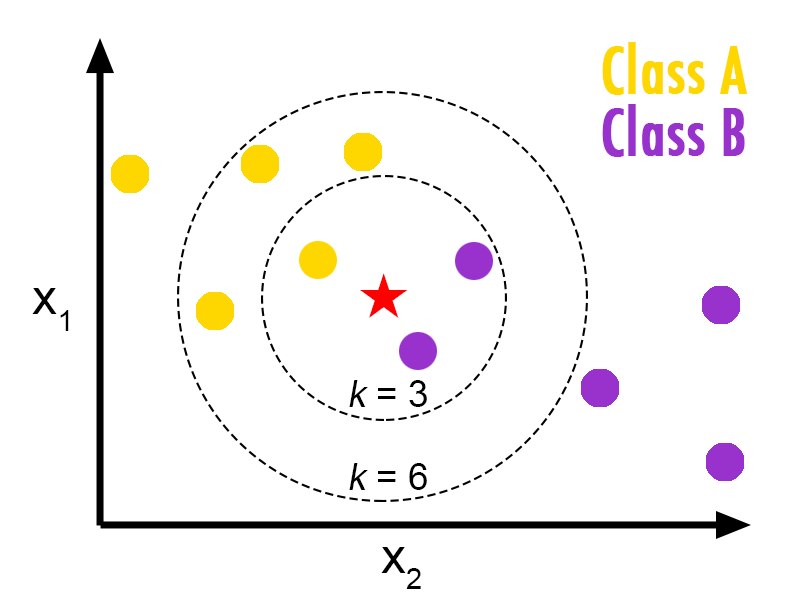
\includegraphics[scale=0.55]{knn-concept.png}
       \caption[caption for kNN]{\label{fig:knnconcept} Visualization of a kNN classifier\footnotemark[1]}
\end{figure}

\footnotetext[1]{Reprinted from GitHub, Burton de Wilde, Retrieved September 13, 2016, from \url{http://bdewilde.github.io/blog/blogger/2012/10/26/classification-of-hand-written-digits-3/}. Copyright 2012 by Burton de Wilde. Reprinted with permission.}

In the case of $k = 10$, $x$ would simply be assigned to the class with the most members. In this case, the training vectors should be given distance-dependent weights (such as $\frac{1}{distance}$) to increase the influence of closer vectors over more distant ones. Hereby, the advantages of the quantum version are the parallel computation of the distances between each training vector and the input vector as well as contracting distance computation and distance weighting into one computational step.

%%% STOPPED SHORTENING HERE!
Next, \cite{Schuld2016} details a quantum algorithm based on linear least-squares regression. In contrast to the discrete classes ($A$ or $B$) used in kNN, this algorithm focusses on continuous outputs and the learning task is to find the best linear fit by reducing the least-squares error to all training data points. A simple example is that in a certain country, given ten data points that link the size of farm land (in ${m}^{2}$) to the total prize (in \$), predict the total prize for a new input size of farm land. Predicting such continuous class labels is important in many fields ranging from medicine to finance. The classical algorithm involves the computation of the (pseudo)inverse of a matrix which becomes computationally intensive for large data sets \citep{decell1975generalized}. In contrast, the runtime of the quantum algorithm is independent of the size of the training data set and mainly depends on the dimension of the training vectors only.

%%CHOOSING SMALL PROBLEMS AND GENERATING THE DATASET
The first step towards implementation of the outlined algorithms will be the identification of one or several small ML problems that can be executed on small-scale quantum computers. For example, this might include the characterization of colours or differentiation of digits or letters. It thereby plays an important role if the respective ML problem can be approached using a very small dataset such as the average pixel brightness or the ratio of pixels above and below the image bisector. Ideally, the data should be representable as a 2-D vector such that it requires only a few qubits to encode the information quantum mechanically.
\newpage
%%THE TOOLS
There are two types of tools available for the implementation of the QML algorithms. Firstly, classical computers can be used to simulate the behaviour of quantum computers. Such simulations are associated with exponential computational costs thereby limiting the number of simulated qubits. Since current state-of-the-art quantum technology uses around ten qubits, a classical computer can still be used for simulation. For example, such a software architecture is provided by Microsoft Research which has released the quantum simulation toolsuite Liqui$\ket{}$ based on the programming language F\#. There are many more QC simulators available and the selection depends on the chosen QML problem and corresponding dataset \citep{quantiki}.

Secondly, earlier this year IBM has enabled public access to their experimental quantum processor containing five non error-corrected superconducting qubits. Instead of only simulating on classical hardware, this opens up the possibility of executing the QML algorithm on actual quantum hardware. Whether it is possible to make use of IBM's QC is highly dependent on the data set chosen. Furthermore, it still remains unclear if the algorithm in \cite{Schuld2016} can be adapted to five qubits since it requires a minimum of six qubits in its current form.

%%THE PROBLEM OF ENCODING THE DATA INTO QUANTUM STATES >> REFERENCE SOME PAPERS HERE
Both algorithms assume that the classical data is readily available in the form of quantum states. Since it is a non-trivial and still researched topic, the first challenge will be translating the classical data into such states. The quantum version of the distance weighted kNN requires a binary data string of length $n$ (e.g. 0110) to be encoded one to one into $n$ qubits (e.g. $\ket{0110}$). This will be referred to as \textit{qubit encoding} and implemented using the algorithm outlined in \cite{ventura1999initializing}.
%The algorithm used for qubit encoding in this research is described in \cite{ventura1999initializing}.
%A possible algorithm for this type of data encoding was proposed by \cite{ventura1999initializing}.
The quantum linear regression algorithm is based on so called \textit{amplitude encoding}, where the classical data is written into the amplitudes ($\alpha$ and $\beta$ in Equ.~\ref{equ: simplequbit}) of quantum states, which is considerably more difficult to achieve than qubit encoding. It is still a very active field of research and so far it can only be done with relatively uniform data sets. For this purpose, the algorithm proposed in \cite{grover2002creating} will be used and special attention will be paid to choosing a suitable dataset.

\begin{figure}[!ht]
      \centering
       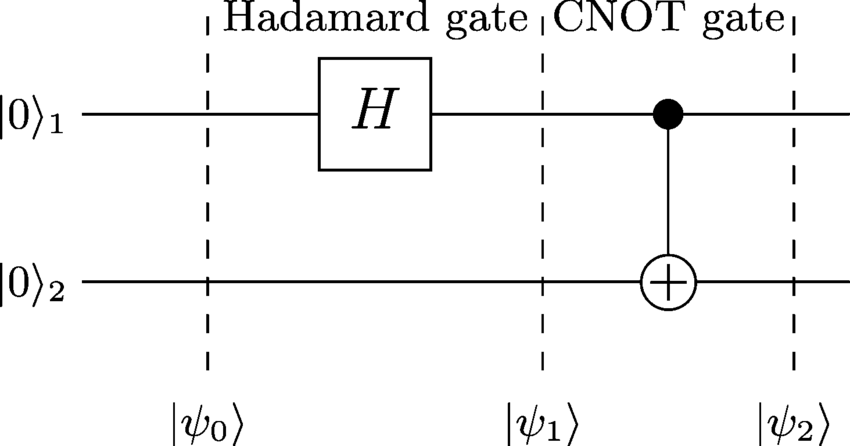
\includegraphics[scale=0.25]{qcircuit.png}
       \caption[caption for qcircuit]{\label{fig:qcircuit} Basic quantum circuit with a single-qubit Hadamard gate (creates a superposition as shown in Equ.~\ref{equ: simplequbit} with $\alpha=\beta=\frac{1}{\sqrt{2}}$) and a two-qubit CNOT gate (controlled bit flip)\footnotemark[2]}
\end{figure}

\footnotetext[2]{Reprinted from \cite{botsinis2013quantum}, Retrieved September 13, 2016, from \url{https://www.researchgate.net/publication/236883187_Quantum_Search_Algorithms_Quantum_Wireless_and_a_Low-Complexity_Maximum_Likelihood_Iterative_Quantum_Multi-User_Detector_Design}. Copyright 2013 by \cite{botsinis2013quantum}. Reprinted with permission.}

%%DESIGNING THE QUANTUM CIRCUITS
Next, two separate quantum circuits consisting of quantum logic gates will be designed that accurately represent the two QML algorithms as outlined in the paper of \cite{Schuld2014, Schuld2016}. Each quantum circuit consist of single- and multi-qubit gates of which a simple example is shown in Fig.~\ref{fig:qcircuit}. Each of those circuits is then combined with its respective quantum data encoding circuit.

Lastly, the computed solution needs to be retrieved by measuring specific qubits. By repeating the execution of the algorithms, a probability distribution of the qubit measurements is obtained that represents the solution to the given problem.
\newpage
To summarize, the steps needed for the successful implementation of a QML algorithm are given below.

\begin{enumerate}
\item Find a small implementable ML problem
\item Generate or find a suitable dataset
\item Encode the classical data into quantum states
\item Design a quantum circuit representing the QML algorithm
\item Execute the entire quantum circuit multiple times
\item Retrieve the solution from the resulting probability distribution
\end{enumerate}

\section{Timeline}
\label{sec:timeline}

The projected timeline for the proposed bachelor thesis research is given below.

\begin{figure}[!ht]
\centering
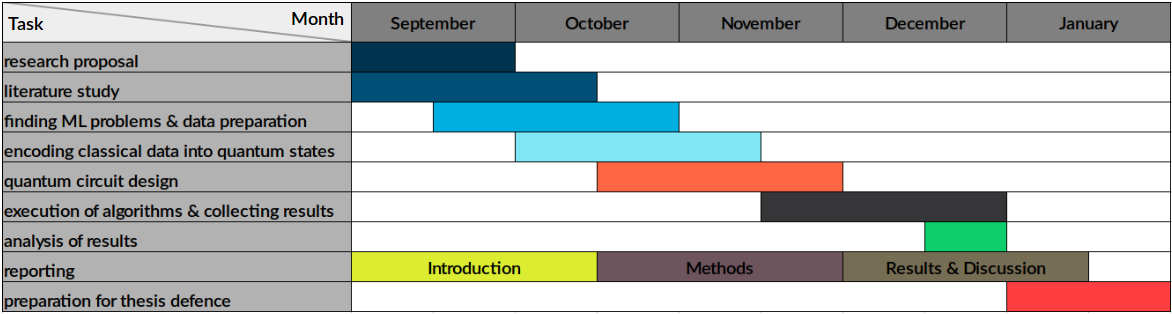
\includegraphics[scale=0.385]{ready_timeline.png}
\caption{Projected timeline for proposed research}
\end{figure}

\section{Research Impact}
\label{sec:research impact}
%is this really needed?
The proposed research is part of the recent effort to move QML from theory to praxis by developing a template for the experimental implementation of the selected QML algorithms. Furthermore, it will provide insights into obstacles such as quantum data representation and error susceptibility. Ideally, the research outcome will demonstrate quantum advantages over the classical algorithms providing supporting evidence for the claim that QML can indeed be used to solve ML problems. Additionally, successful proof-of-concept studies are crucial for further research to be funded and supported since it shows that an upscaling of quantum computational power will eventually lead up to exponential speed-ups compared to classical ML and hence has the potential to revolutionize the handling of big data.

\section{Conclusion}
\label{sec:conclusion}
Recently, many inventive and powerful improvements to classical ML algorithms were published in the field of QML. Such algorithms are required in order to cope with and make sense of the enormous amounts of data generated in contemporary society. However, the required computational resources are not available yet and proof-of-concept studies are needed to further stress the value of theoretical developments in QML. The proposed research will identify small ML problems and suitable datasets that can already be solved using QML algorithms on small-scale quantum computers. Investigated will be two algorithms given in \cite{Schuld2014, Schuld2016} which focus on supervised pattern classification based on linear regression and kNN. The key steps will be encoding the classical data into quantum states and designing quantum circuits representing the algorithms. Possible tools for the research include IBM's five-qubit quantum processor or QC simulators executed on a classical computer.

\section{References}
\begingroup
\renewcommand{\section}[2]{}%
\bibliographystyle{apacite}
\bibliography{proposal}
\endgroup

%\newpage

%\section{Appendix}


\end{document}